\documentclass[letter, 11pt]{article}
\usepackage{fullpage}
\usepackage[margin=0.5in]{geometry}
\usepackage{graphicx}
\usepackage{caption}
\usepackage{subcaption}
\usepackage{amsmath}
\usepackage{listings}
\usepackage{float}
\usepackage{array,multirow}
\usepackage{tikz}
\usetikzlibrary{arrows}
\pagenumbering{gobble}
\begin{document}
\noindent
\large \textbf{Rahul Ghosh} \hfill \textbf{Assignment\#1}\\
\normalsize Student ID: 5476965 \hfill CSci 5512\\

\section*{Question 1}
\setcounter{equation}{0}
According to normalization,
\begin{align}
    & P(a|b) = \alpha P(a,b)
\end{align}
We know that,
\begin{align}
    & P(a|b) + P(\neg a|b) = 1\notag\\
    & \alpha P(a,b) + \alpha P(\neg a,b) = 1 \qquad from (1)\notag\\
    & \alpha P(b) = 1\notag\\
    & P(b) = \frac{1}{\alpha}
\end{align}
Now,
\begin{align}
    & P(a|b)=\alpha P(a,b)\notag\\
    \implies & P(a|b)=\alpha P(b|a)P(a)\notag\\
    \implies & P(a|b) = \frac{P(b|a)P(a)}{P(b)} \qquad from (2)
\end{align}
But equation(3) is also the Bayes Theorem. Therefore instead of dividing by $P(b)$, we can also find $P(\neg a|b)$ and normalize

\section*{Question 2}
\setcounter{equation}{0}
\begin{itemize}
    \item[(1)] $0 \leq P(\omega) \leq 1$
    \item[(2)] $\sum_{\omega \epsilon \Omega} P(\omega)=1$
    \item[(3)] $P(a) + P(\neg a) = 1$
    \item[(4)] $P(a\ or\ b) = P(a) + P(b) - P(a,b)$
    \item[(5)] $P(a) = \sum_{b} P(a,b)$
\end{itemize}
Given: P(a) = 0.2, P(b) = 0.3, P(a or b)=0.1\\
Proof: Using (4) we get, 
\begin{align}
    P(a,b) = 0.4\notag
\end{align}
From (1), we know that $P(\omega)$ is a non-negative number.\\
Therefore, from (5)
\begin{align}
    P(a) \geq P(a,b) \And P(b) \geq P(a,b) \notag
\end{align}
But from the values we get that,
\begin{align}
    P(a) < 0.4 \And P(b) < 0.4\notag
\end{align}
Thus the probabilities are not consistent with each other.

\section*{Question 3}
\setcounter{equation}{0}
\begin{itemize}
    \item[(1)] P(a,b)
        \begin{flalign*}
            P(a,b) &= \sum_{c} P(a,b,c)&\\
                    &= P(a,b,c) + P(a,b,\neg c)&\\
                    &= 0.018837 + 0.011063&\\
                    &= 0.0299
        \end{flalign*}
    \item[(2)] P(a,b$|$c)
        \begin{flalign*}
            P(c) &= \sum_{a,b} P(a,b,c)&\\
                &= P(a,b,c)+P(\neg a,b,c)+P(a,\neg b,c)+P(\neg a,\neg b, c)&\\
                &= 0.018837+0.126324+0.063063+0.160776&\\
                &=0.369&\\
            P(a,b|c) &= \frac{P(a,b,c)}{P(c)}&\\
                    &= \frac{0.018837}{0.369}&\\
                    &= 0.051
        \end{flalign*}
    \item[(3)] P(c$|\neg$a)
        \begin{flalign*}
            P(\neg a,c) &= \sum_{b} P(\neg a,b,c)&\\
                &= P(\neg a,b,c)+P(\neg a,\neg b,c)&\\
                &= 0.126324 + 0.160776&\\
                &=0.2871&\\
            P(\neg a) &= \sum_{b,c} P(\neg a,b,c)&\\
                    &= 0.8700&\\
            P(c|\neg a) &= \frac{P(\neg a,c)}{P(\neg a)}&\\
                        &= 0.22871/0.87&\\
                        &=0.330
        \end{flalign*}
    \item[(4)] P(b)
        \begin{flalign*}
            P(b) &= P(a,b,c)+P(\neg a,b,c)+P(a,b,\neg c)+P(\neg a,b,\neg c)&\\
                &= 0.018837+0.126324+0.011063+0.256476&\\
                &= 0.4127
        \end{flalign*}
\end{itemize}

\section*{Question 4}
\setcounter{equation}{0}
\begin{flalign}
    &P(a)\times P(b) = 0.1300 \times 0.4127 = 0.0537&\\
    &P(a,b) = 0.0299&\\
    &P(a)\times P(c) = 0.1300 \times 0.3690 = 0.0480&\\
    &P(a,c) = 0.0819&\\
    &P(b)\times P(c) = 0.4127 \times 0.3690 = 0.1523&\\
    &P(b,c) = 0.1452
\end{flalign}
Since $(1)\neq(2), (3)\neq(4) \And (5)\neq(6)$, none of the variables are independent.
\begin{flalign}
    &P(a|c)\times P(b|c) = 0.2220 \times 0.3934 = 0.0873&\\
    &P(a,b|c) = 0.0510&\\
    &P(a|b)\times P(c|b) = 0.0724 \times 0.3517 = 0.0255&\\
    &P(a,c|b) = 0.0456&\\
    &P(b|a)\times P(c|a) = 0.2300 \times 0.6300 = 0.1449&\\
    &P(b,c|a) = 0.1449
\end{flalign}
Since $(11)=(12)$, b and c are conditionally independent.

\section*{Question 5}
\setcounter{equation}{0}
\begin{itemize}
    \item[(1)] Let the variable order be A, B and C.\\
    \begin{itemize}
        \item[-] First loop iteration, we need to find, P(A$|$Parent(A)). But since i=1, no parents needed to be found.
                \begin{equation*}
                    P(A|nothing) = P(A)
                \end{equation*}
        \item[-] Next loop iteration, We find P(B$|$Parent(B)) for which we have two options,
                \begin{equation*}
                    P(B|A) = \begin{cases}
                                P(B|A)\\
                                P(B)
                            \end{cases}
                \end{equation*}
                But since B and A are not independent, the second options is not possible. So Parent(B)=A
        \item[-] Last iteration we find, P(C$|$Parent(C)),
                \begin{equation*}
                    P(C|Parent(C)) = P(C|B,A) 
                \end{equation*}
                but since C and B are conditionally independent,
                \begin{equation*}
                    \implies P(C|Parent(C)) = P(C|B,A) = P(C|A)
                \end{equation*}
                So Parent(C)=A
    \end{itemize}
    So depending on this network we have,\\
    \begin{tabular}{ |c|c|c| } 
        \hline
        \multirow{2}{*}{P(a)=0.1300} & P(b$|$a) = 0.2300 & P(c$|$a) = 0.6300 \\\cline{2-3}
        & P(b$|\neg$a) = 0.4400 & P(c$|\neg$a) = 0.3300 \\\cline{3-3}
        \hline
    \end{tabular}
    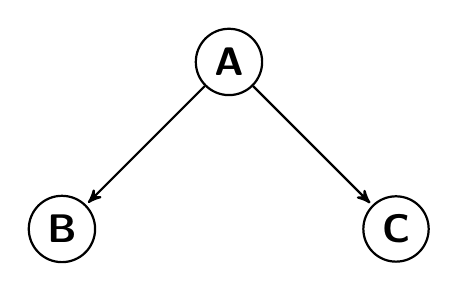
\begin{tikzpicture}[baseline={(current bounding box.east)},->,>=stealth',shorten >=1pt,auto,node distance=3cm,thick,main node/.style={circle,draw,font=\sffamily\Large\bfseries}]

        \node[main node] (1) {A};
        \node[main node] (2) [below left of=1] {B};
        \node[main node] (3) [below right of=1] {C};
        
        \path[every node/.style={font=\sffamily\small}]
        (1) edge node {} (3)
            edge node {} (2);
    \end{tikzpicture}
    
    \item[(2)] Let the variable order be C, B and A.\\
    \begin{itemize}
        \item[-] First loop iteration, we need to find, P(C$|$Parent(C)). But since i=1, no parents needed to be found.
                \begin{equation*}
                    P(C|nothing) = P(C)
                \end{equation*}
        \item[-] Next loop iteration, We find P(B$|$Parent(B)) for which we have two options,
                \begin{equation*}
                    P(B|C) = \begin{cases}
                                P(B|C)\\
                                P(B)
                            \end{cases}
                \end{equation*}
                But since B and C are not independent, the second options is not possible. So Parent(B)=C
        \item[-] Last iteration we find, P(A$|$Parent(A)),
                \begin{equation*}
                    P(A|Parent(A)) = P(A|B,C) 
                \end{equation*}
    \end{itemize}
    So depending on this network we have,\\
    \begin{tabular}{ |c|c|c| } 
        \hline
        \multirow{4}{*}{P(c)=0.3690} & \multirow{2}{*}{P(b$|$c) = 0.3934} & P(a$|$b,c) = 0.1298 \\\cline{3-3}
        & & P(a$|\neg$b,c) = 0.2817 \\ \cline{2-3}
        & \multirow{2}{*}{P(b$|\neg$c) = 0.4240} & P(a$|$b,$\neg$c)=0.0414 \\\cline{3-3}
        & & P(a$|\neg$b,$\neg$c)=0.1019 \\
        \hline
    \end{tabular}
    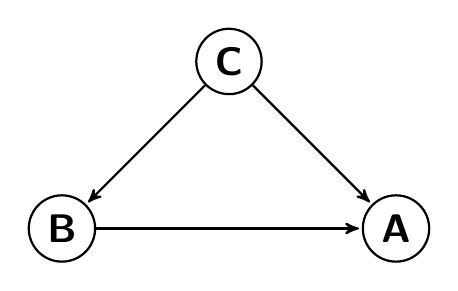
\begin{tikzpicture}[baseline={(current bounding box.east)},->,>=stealth',shorten >=1pt,auto,node distance=3cm,thick,main node/.style={circle,draw,font=\sffamily\Large\bfseries}]

        \node[main node] (C) {C};
        \node[main node] (B) [below left of=C] {B};
        \node[main node] (A) [below right of=C] {A};
        
        \path[every node/.style={font=\sffamily\small}]
        (C) edge node {} (B)
            edge node {} (A)
        (B) edge node {} (A);
    \end{tikzpicture}
    
\end{itemize}
\section*{Question 6}
\setcounter{equation}{0}
\begin{itemize}
    \item[(1)] let the "slot reward" be the random variable. According to the given information,
    \begin{flalign*}
        &P(slot\_reward = 100) = 0.1&\\
        &P(slot\_reward = 30) = 0.3&\\
        &P(slot\_reward = 5) = 0.5&\\
        &P(slot\_reward = 0) = 0.1
    \end{flalign*}
    \item[(2)] Using the above probabilities the expected reward from the slot machine is,
    \begin{align*}
        E[reward] &= \sum reward*P(reward)&\\
        &= (100*0.1)+(30*0.3)+(5*0.5)+(0*0.1)&\\
        &= 10+9+2.5&\\
        &= 21.5
    \end{align*}
    Therefore the Casino should attach \$21.5 to play at this machine.
    \item[(3)]
    \begin{align*}
        P(atleast\ 1\ reward) &= 1-P(no\ reward)&\\
        &= 1-(0.1)^5&\\
        &= 1-0.00001&\\
        &= 0.99999
    \end{align*}
\end{itemize}

\section*{Question 7}
\setcounter{equation}{0}
\begin{flalign*}
    E[reward] = &\sum reward*P(reward)&\\
    = &(100+0)(0.1)(0.5) + (100+5)(0.1)(0.5)+&\\
    &(30+0)(0.3)(0.1)+(30+5)(0.3)(0.5)+(30+30)(0.3)(0.3)+(30+100)(0.3)(0.1)+&\\
    &(5+0)(0.5)(0.1)+(5+5)(0.5)(0.5)+(5+30)(0.5)(0.3)+(5+100)(0.5)(0.1)+&\\
    &(0+0)(0.1)(0.1)+(0+5)(0.1)(0.5)+(0+30)(0.1)(0.3)+(0+100)(0.1)(0.1)&\\
    =&5 + 5.25 + 0.9 + 5.25 + 5.4 + 3.9 + 0.25 + 2.5 + 5.25 + 5.25 + 0 + 0.25 + 0.9 + 1&\\
    = &41.1
    \end{flalign*}


\end{document}